\documentclass[9pt,a9paper,handout]{beamer}
\usepackage[T1]{fontenc}
\usepackage[utf8]{inputenc}
\usepackage[francais]{babel}
\usepackage{amsmath,amsfonts,amssymb,tikz,colortbl,lmodern,xspace,subfigure}
\usepackage{siunitx,array,url} % Symboles, etc
\usetheme{Berlin}
\usecolortheme{seagull}
\setbeamertemplate{caption}{\raggedright\insertcaption\par}
\setcounter{tocdepth}{1}

\defbeamertemplate*{footline}{myfootline} {
  \leavevmode%
  \hbox{%
      \begin{beamercolorbox}[wd=.32\paperwidth,ht=3ex,dp=1ex,left]{title in head/foot}%
        \scriptsize\hspace{4px}\insertshortauthor
      \end{beamercolorbox}%
      \hspace*{-5px}
      \begin{beamercolorbox}[wd=.34\paperwidth,ht=3ex,dp=1ex,center]{title in head/foot}%
%        \scriptsize\insertshortinstitute
      \end{beamercolorbox}%
      \hspace*{-5px}
      \begin{beamercolorbox}[wd=.36\paperwidth,ht=3ex,dp=1ex,right]{title in head/foot}%
        \scriptsize\insertshortdate{}\hspace*{2em}
        \scriptsize\insertframenumber{} / \inserttotalframenumber\hspace*{2ex} 
      \end{beamercolorbox}
  }%
  \vskip0pt%
}
\defbeamertemplate*{title page}{customized}[1][]
{
  \vbox{}
  \vfill
  \begingroup
    \centering
    \begin{beamercolorbox}[sep=8pt,center,#1]{title}
      \usebeamerfont{title}\inserttitle\par%
      \ifx\insertsubtitle\@empty%
      \else%
        \vskip0.25em%
        {\usebeamerfont{subtitle}\usebeamercolor[fg]{subtitle}\insertsubtitle\par}%
      \fi%     
    \end{beamercolorbox}%
    \vskip1em\par
    \begin{beamercolorbox}[sep=8pt,center,#1]{author}
      \usebeamerfont{author}\insertauthor
    \end{beamercolorbox}
    \begin{beamercolorbox}[sep=8pt,center,#1]{institute}
      \usebeamerfont{institute}\normalsize \insertinstitute
    \end{beamercolorbox}
    \begin{beamercolorbox}[sep=8pt,center,#1]{date}
      \usebeamerfont{date}\insertdate
    \end{beamercolorbox}\vskip0.5em
    {\usebeamercolor[fg]{titlegraphic}\inserttitlegraphic\par}
  \endgroup
  \vfill
}
\defbeamertemplate*{headline}{myheadline} {
    \begin{beamercolorbox}[colsep=1.5pt]{upper separation line head}
    \end{beamercolorbox}
    \begin{beamercolorbox}{section in head/foot}
    \vskip2pt\insertnavigation{\paperwidth}\vskip2pt
    \end{beamercolorbox}%
    \begin{beamercolorbox}[colsep=1.5pt]{lower separation line head}
    \end{beamercolorbox}
}


\makeatother
\setbeamertemplate{footline}[myfootline]

\title{Caractérisation de pointes fibrées dans l'optique d'une nano-pince optique plasmonique}
\author{Félix Piédallu}
\date{29 Juin 2016}
\institute{Grenoble INP Phelma, Filière Physique - Nanosciences\\Institut Néel - Équipe NanoOptique et Forces}

\begin{document}

\begin{frame}
    \maketitle
    \begin{center}
        \vspace*{6mm}
        
\includegraphics[width=50px]{Images/logo_phelma}
        \hspace*{4cm}
        
\includegraphics[width=50px]{Images/logo_neel}
        %
\includegraphics[width=40px]{Images/logo_cnrs}\qquad
        \\[0.2cm]
        Sous la direction de Jochen Fick
    \end{center}
\end{frame}


\section{Contexte du stage}
    % Présentation de la pince optique
    \begin{frame}
        \frametitle{Contexte du stage: Les pinces optiques}
        
        \begin{columns}[T]
        \begin{column}{0.70\textwidth}
        \begin{itemize}
            \vspace*{8mm}
            \item Faisceau focalisé (objectif de microscope)
            \vspace*{10mm}
            \item Faisceau collimaté (pointes fibrées): \\intégration et manipulations plus faciles
        \end{itemize}
        \vspace*{-5mm}
        \begin{figure}[H]
            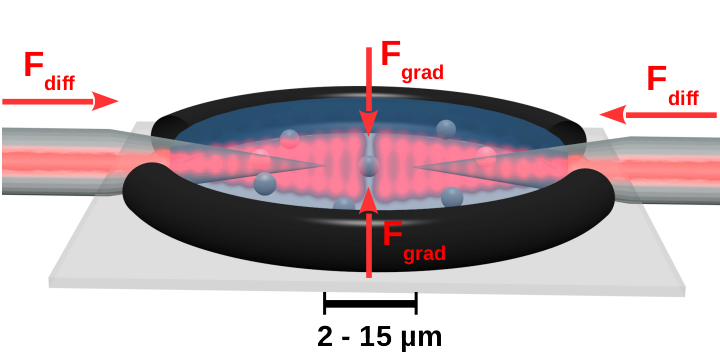
\includegraphics[width=0.7\textwidth]{Images/Schemas/piegeage_deuxpointes}
        \end{figure}
        \end{column}
        \begin{column}{0.3\textwidth}
            \begin{figure}[H]
                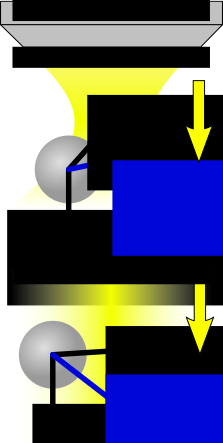
\includegraphics[width=0.82\textwidth]{Images/Schemas/FaisceauConfinement}
            \end{figure}
        \end{column}
        \end{columns}


    \vspace*{5mm}
        {\large $\rightarrow$ Caractérisation des pointes} \vspace*{1mm}\\
        \qquad Caractérisation spatiale et spectrale de l'émission

    \end{frame}


\section{Élaboration des pointes}
    \begin{frame}
        \frametitle{Élaboration des pointes fibrées}
        \begin{itemize}
            \item Gravure chimique en pointe\\
            \qquad "Tube Etching" au HF
        \end{itemize}

        \begin{figure}[h]\centering
            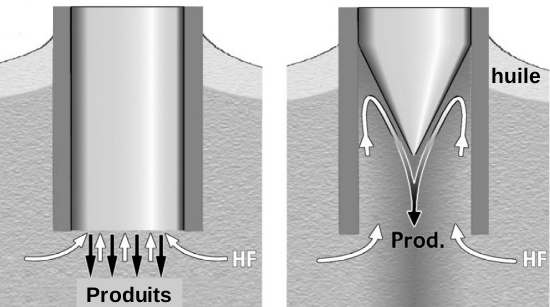
\includegraphics[width=.4\textwidth]{Images/Schemas/gravure}
            \hspace*{3mm}
            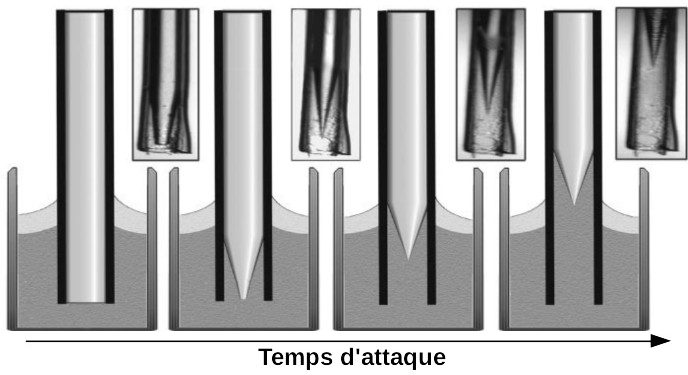
\includegraphics[width=.4\textwidth]{Images/Schemas/gravure_2}
        \end{figure}
        \vspace*{1cm}

        \begin{figure}[h]\centering
            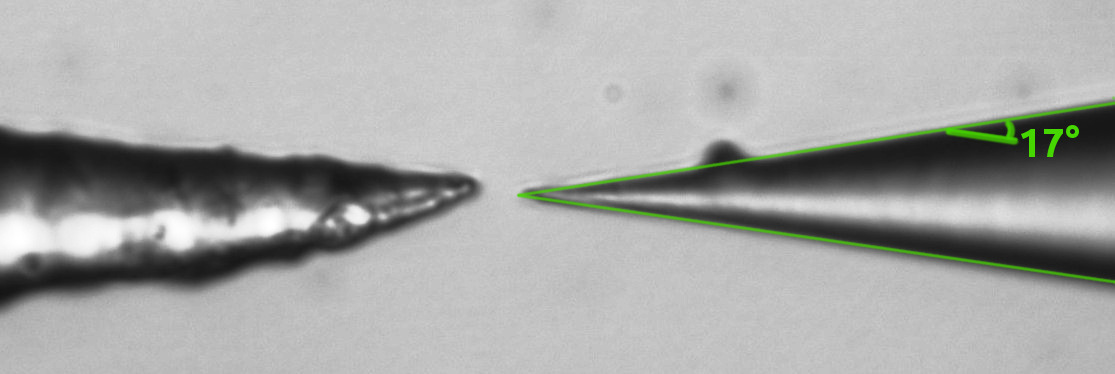
\includegraphics[width=.55\textwidth]{Images/PhotosPointes/Nues_ok_et_abimee}
        \end{figure}
    \end{frame}

    \begin{frame}
        \frametitle{Métallisation des pointes}
        \begin{itemize}
            \item Dépôt métallique par évaporation
            \begin{itemize}
                \item couche d'accroche de Titane
                \item couche d'or (40nm - 150nm)
            \end{itemize}
            \vspace*{3mm}
                \begin{figure}[h]\centering
                    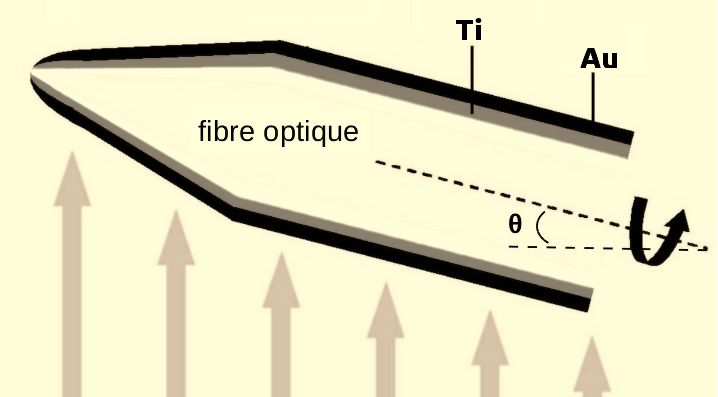
\includegraphics[width=.4\textwidth]{Images/Schemas/evaporation_metal}
                \end{figure}

            \item Découpe au FIB, contrôle au MEB
        \end{itemize}
        \begin{figure}[h]\centering
            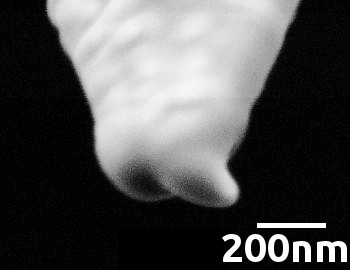
\includegraphics[width=.25\textwidth]{Images/PhotosPointes/l33fm2_avant_crop}
            \hspace*{3mm}
            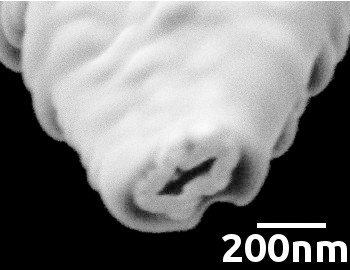
\includegraphics[width=.25\textwidth]{Images/PhotosPointes/l33fm2_apres_crop}
        \end{figure}
    \end{frame}


\section{Matériel expérimental}
    \begin{frame}
        \frametitle{Chemin optique}
        \begin{figure}\centering
            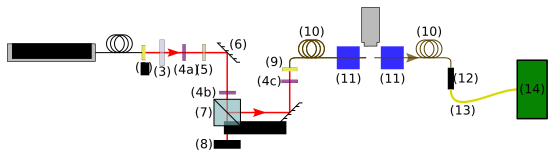
\includegraphics[width=0.8\textwidth]{Images/Schemas/experience}
        \end{figure}
        \begin{itemize}
            \item Faisceau laser gaussien à $\lambda = 808nm$
            \item Contrôle en intensité et polarisation
            \item Positionnement sub-nanométrique
            \item Observation au microscope
        \end{itemize}
    \end{frame}

    \begin{frame}
        \frametitle{Positionnement des pointes fibrées}
        \begin{figure}\centering
            %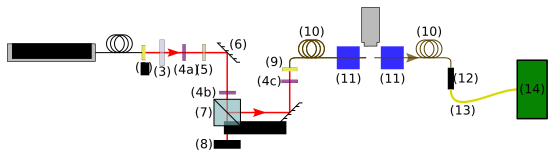
\includegraphics[width=0.8\textwidth]{Images/Schemas/experience}
            \caption{[TODO] Photo mechonics - fibres dans l'eau - PI, de dessus}
        \end{figure}
        \begin{itemize}
            \item Moteurs piezoélectriques inertiels: positionnement des fibres
            \item Platines piezoélectriques: alignement et balayage sub-nanométriques
        \vspace*{2mm}
            \item Cavité de Fabry-Pérot: asservissement en position
        \end{itemize}
        \vspace*{3mm}
        \begin{minipage}{\textwidth}
            \centering
            \raisebox{-0.5\height}{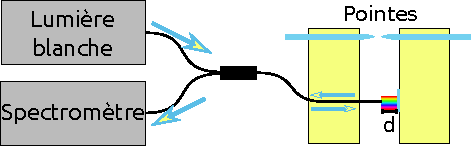
\includegraphics[width=0.35\textwidth]{Images/Schemas/SpectroDistance}}
            \hspace*{3mm}
            \raisebox{-0.5\height}{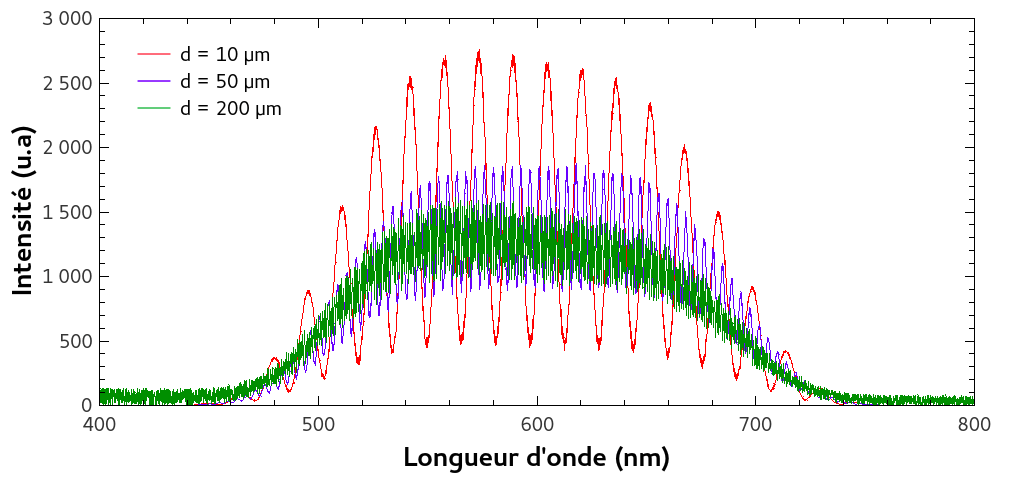
\includegraphics[width=0.35\textwidth]{Images/Schemas/SpectroDistance_plot}}
        \end{minipage}
    \end{frame}

    \begin{frame}
        \frametitle{Observation des fibres}
        \begin{itemize}
            \item Imagerie MEB
        \end{itemize}
        \vspace*{-1cm}
        \begin{figure}\flushright
            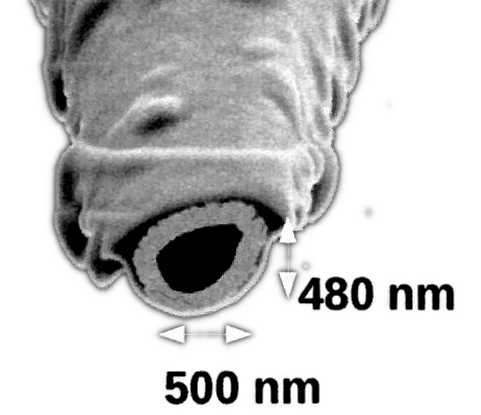
\includegraphics[width=0.3\textwidth]{Images/PhotosPointes/photo_meb_exemple}
        \end{figure}
        
        \begin{itemize}
            \item Microscopie en champs clair et sombre
        \end{itemize}
        \vspace*{3mm}
        \begin{minipage}{\textwidth}
            \centering
            \raisebox{-0.5\height}{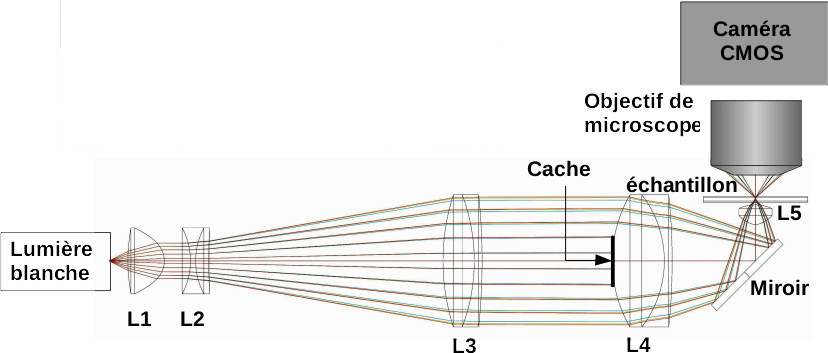
\includegraphics[width=0.5\textwidth]{Images/Schemas/champ_sombre}}
            \hspace*{3mm}
            \raisebox{-0.5\height}{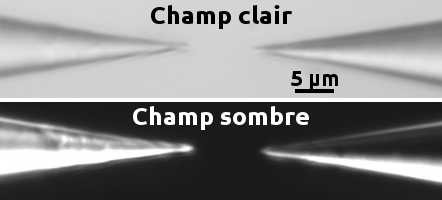
\includegraphics[width=0.45\textwidth]{Images/PhotosPointes/champs_clair_sombre}}
        \end{minipage}
    \end{frame}



\section{Émission spatiale des pointes}
    \begin{frame}
        \frametitle{Émission spatiale des pointes}
        Scans en (y, z) de l'émission d'une pointe grâce à une autre pointe
        \begin{figure}[c]\centering
            
\includegraphics[width=0.6\textwidth]{Images/Schemas/FibresScan}
        \end{figure}
        \vspace*{1mm}
        \begin{itemize}
            \item Mesure de l'angle d'émission des pointes \textbf{non métallisées}
            \begin{itemize}
                \item Dans l'air: 18\si{\degree} $\rightarrow$ $N.A=0.16$
                \item Dans l'eau:  8\si{\degree} $\rightarrow$ $N.A=0.09$
            \end{itemize}
        \end{itemize}
        \vspace*{-6mm}
        \begin{figure}[c]\flushright
            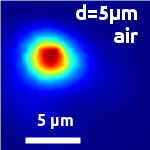
\includegraphics[height=0.15\textwidth]{Images/Scans/Spot_small}
            \quad
            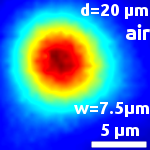
\includegraphics[height=0.15\textwidth]{Images/Scans/Spot_big}
            \quad
            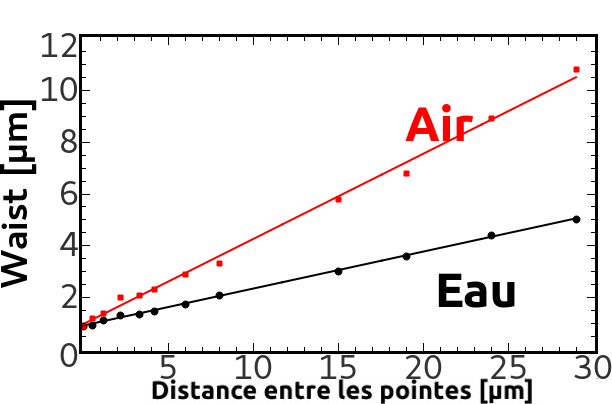
\includegraphics[height=0.20\textwidth]{Images/Scans/NuesDistanceWaist}\\
            ~\\
            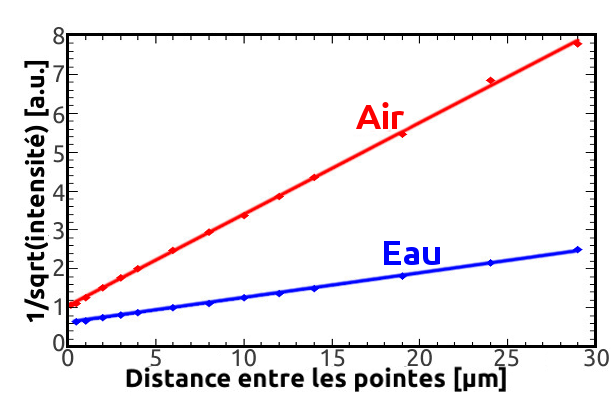
\includegraphics[height=0.195\textwidth]{Images/Scans/NuesDistanceIntensite}
        \end{figure}
        \vspace*{-15mm}
        \begin{itemize}
            \item Intensité plus élevée dans l'eau que dans l'air
        \end{itemize}
    \end{frame}


    \begin{frame}    
        \frametitle{Émission spatiale des pointes de Bessel}
        {\large Pointe et faisceau de Bessel}
        \vspace*{-2mm}\\
        \begin{figure}[H]
            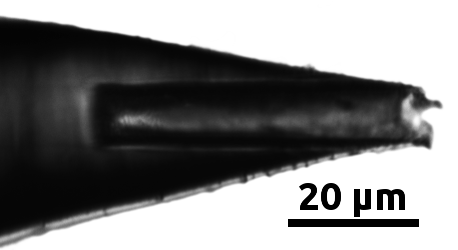
\includegraphics[width=0.20\textwidth]{Images/PhotosPointes/Bessel_1}
            \qquad
            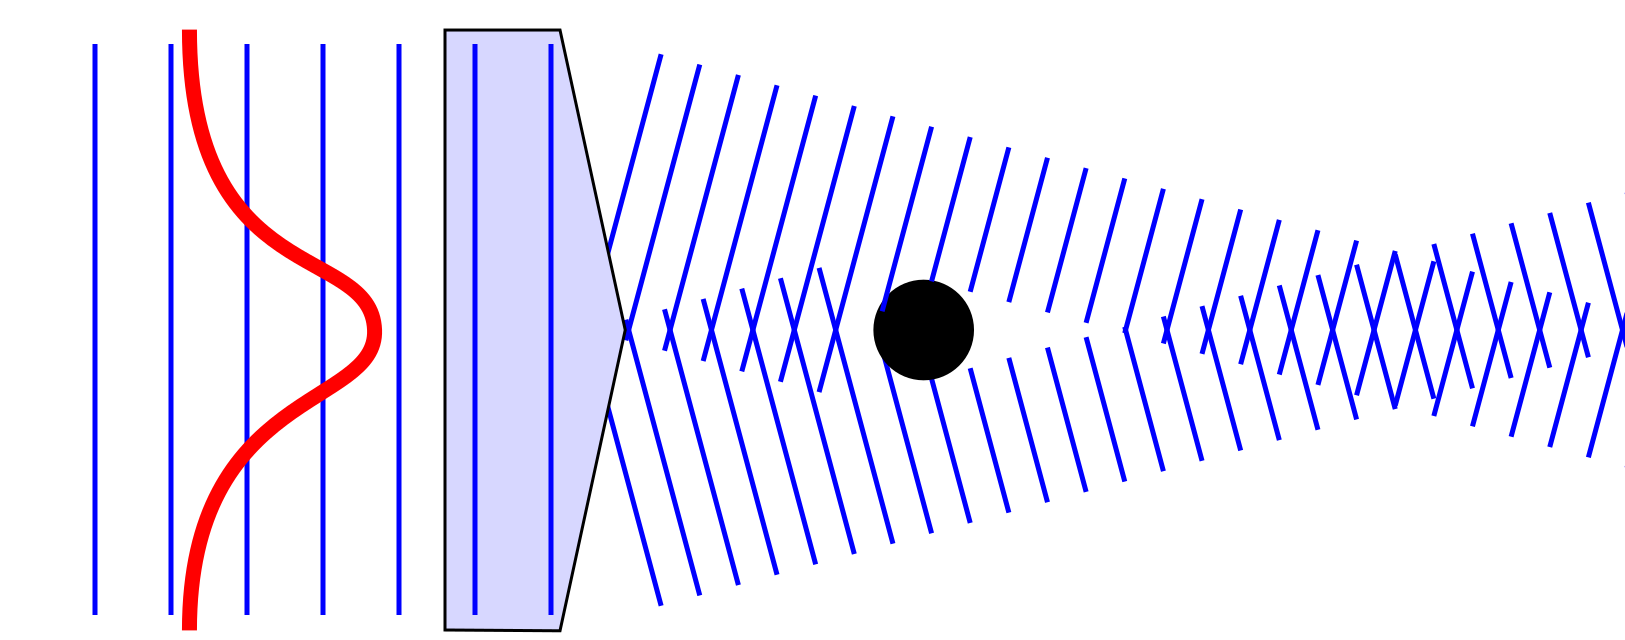
\includegraphics[width=0.40\textwidth]{Images/Schemas/bessel}
        \end{figure}

        \vspace*{4mm}
        {\large Profil d'émission et évolution spatiale} \vspace*{1mm}\\
        \begin{figure}[t]\centering
            \vspace*{-3mm}
            \includegraphics[width=0.15\textwidth]{{"Images/Scans/bessel_5um"}}
            \;
            \includegraphics[width=0.35\textwidth]{{"Images/Scans/bessel_courbe"}}
            \;
            \includegraphics[width=0.15\textwidth]{{"Images/Scans/bessel_90um"}}
        \end{figure}

        \begin{itemize}
            \item Angle d'émission : $\theta = 0.47\si\degree \rightarrow N.A = 0.005$
                \begin{itemize}
                    \item Grande distance de travail
                \end{itemize}
            \item Faisceau "auto-réparant"
        \end{itemize}
        \let\thefootnote\relax\footnotetext{Samir R. Mondal, \textit{Central Scientific Instruments Organization} à Chandigarh (Inde)}
    \end{frame}

    \begin{frame}    
        \frametitle{Émission spatiale des pointes métallisées}
        \begin{figure}[c]\centering
            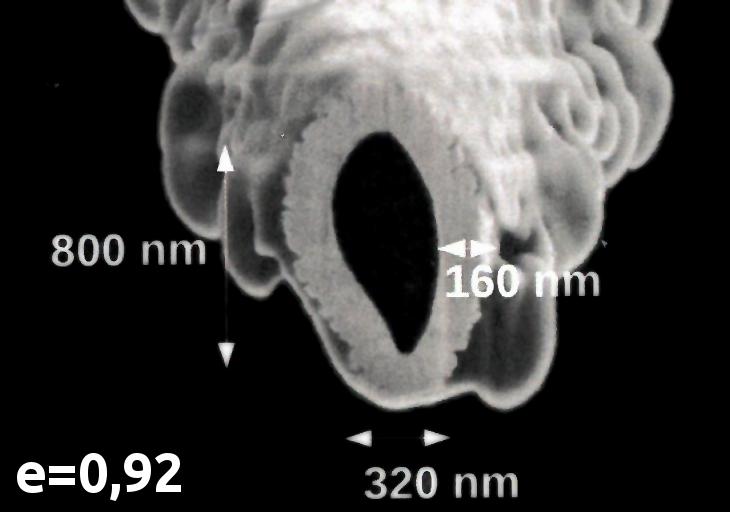
\includegraphics[height=0.13\textwidth]{Images/PhotosPointes/pointe_metallisee_injection}
            \;
            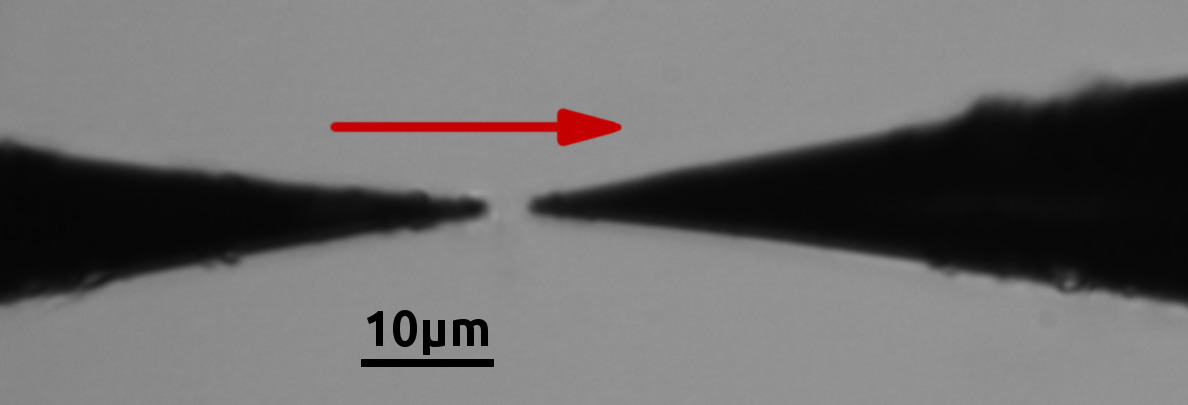
\includegraphics[height=0.13\textwidth]{Images/PhotosPointes/pointes_metallisees}
            \;
            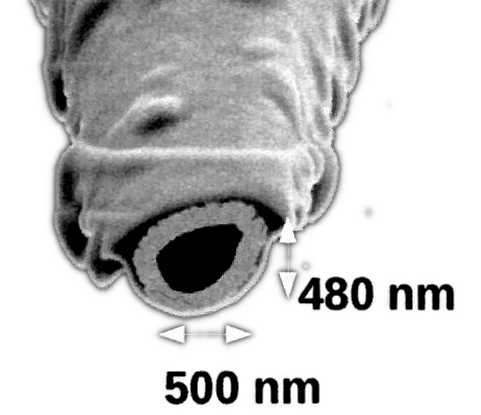
\includegraphics[height=0.13\textwidth]{Images/PhotosPointes/photo_meb_exemple}
        \end{figure}

        \begin{itemize}
            \item Faible distance
        \end{itemize}
    \vspace*{-6mm}
        \begin{figure}[c]\flushright
            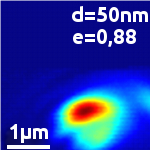
\includegraphics[height=0.15\textwidth]{Images/Scans/Metal_50nm}
            \quad
            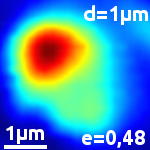
\includegraphics[height=0.15\textwidth]{Images/Scans/Metal_1um}
            \quad
            \raisebox{-4mm}{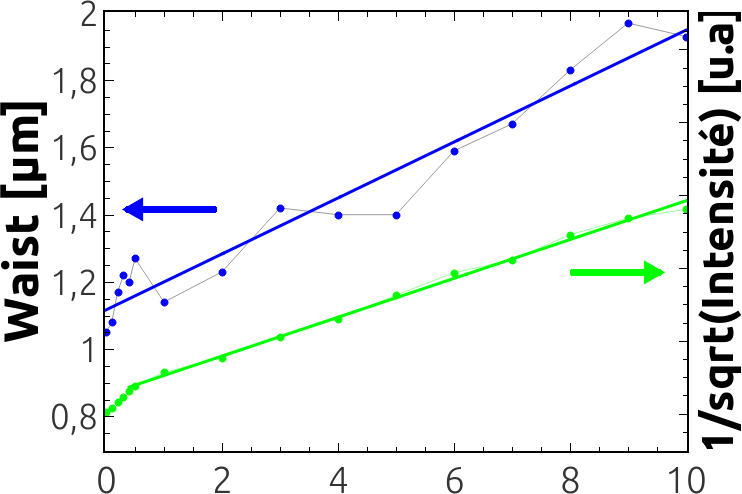
\includegraphics[height=0.22\textwidth]{Images/Scans/DistanceMetal}}
        \end{figure}
    \vspace*{5mm}

        \begin{itemize}
            \item Forte dépendance en polarisation incidente
        \end{itemize}
    \vspace*{-8mm}
        \begin{figure}[c]\flushright
            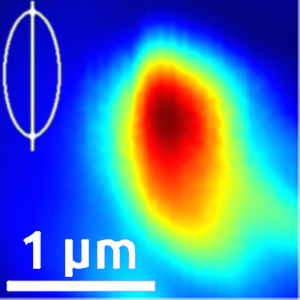
\includegraphics[height=0.15\textwidth]{Images/Scans/polar_long_2}
            \quad
            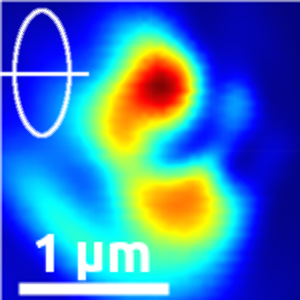
\includegraphics[height=0.15\textwidth]{Images/Scans/polar_trans}\\
            d=80nm
        \end{figure}
    \end{frame}



\section{Émission spectrale des pointes}
    \begin{frame}
        \frametitle{Émission spectrale des pointes}
        
        \begin{columns}[T]
        \begin{column}{0.60\textwidth}
            {\large Injection de lumière blanche}
            \begin{itemize}
                \item Spectres en transmission
                \begin{itemize}
                    \item Pointe non métallisée
                    \includegraphics[width=0.7\textwidth]{{"Images/Schemas/Spectro_nue_nue"}}
                    \item Pointe métallisée (ouverture $\varnothing \simeq 950nm$)
                    \includegraphics[width=0.7\textwidth]{{"Images/Schemas/Spectro_metal_nue"}}
                \end{itemize}
                \vspace*{1cm}
                \item Meilleure transmission dans l'eau
                \vspace*{1cm}
                \item Longueur d'onde de coupure pour les fibres métallisées
            \end{itemize}
        \end{column}
        \begin{column}{0.4\textwidth}\flushright
            \begin{figure}[h]
                    \includegraphics[width=0.98\textwidth]{{"Images/Spectro/Intensite_toutes"}}
            \end{figure}
            \begin{figure}[h]
                    \includegraphics[width=\textwidth]{{"Images/Spectro/Transmission_toutes"}}
            \end{figure}

        \end{column}
        \end{columns}

    \end{frame}

\begin{frame}
    \frametitle{Conclusion}
    \begin{itemize}
        \item Pointes non métallisées utilisables en champ lointain
        \item Pointes de Bessel utilisables à très grande distance
        \item Couplage plasmonique dans les pointes métallisées en champ proche
    \end{itemize}
\end{frame}

\begin{frame}
    \begin{LARGE}
    \begin{center}
    \textbf{Merci de votre attention !}
    \vspace{0.5cm}
    
    \textbf{N'hésitez pas si vous avez des questions.}
    \end{center}
    \end{LARGE}
\end{frame}
\end{document}
